%%%%%%%%%%%%%%%%%%%%%%%%%%%%%%%%%%%%%%%%%%%%%%%%%%%%%%%%%%%%%%%%%%%%%%%%%%%%%%%%
% TUM-Vorlage: Präsentation - Beispiele
%%%%%%%%%%%%%%%%%%%%%%%%%%%%%%%%%%%%%%%%%%%%%%%%%%%%%%%%%%%%%%%%%%%%%%%%%%%%%%%%

\begin{frame}
	\frametitle{\LARGE Implementation of Membranes}
	\large
	\begin{itemize}
		\item Membrane is wrapper class around 2D-vector of Particle IDs
		\item Actual Particles still get stored in ParticleContainer
	\end{itemize}

	\vspace{1cm}

	\LARGE
	Implementation of immovable Particles
	\large
	\begin{itemize}
		\item Set mass of particle to -inf
		\item refactor code to ignore those particles wherever needed (e.g. Thermostat)
	\end{itemize}
	
\end{frame}

%\begin{frame}
%	\frametitle{Implementation of immovable Particles}
%	\large
%	\begin{itemize}
%		\item Set mass of particle to -inf
%		\item refactor code to ignore those particles wherever needed (e.g. Thermostat)
%	\end{itemize}
%\end{frame}

\begin{frame}
	\frametitle{Preparation for Multithreading- Refactoring the Particle Container}
	\large
	Our current implementation of the Cell Data structure (as displayed in Assigment 3):
	\vspace{-0.3cm}
	\begin{itemize}
		\item Particles get stored in one giant vector
		\item Each Cell keeps references to their particles
		\item No sorting or copying takes place
	\end{itemize}
	\vspace{-0.1cm}
	
	\begin{columns}
		\begin{column}{0.5\textwidth}
	\begin{tikzpicture}
		%define constants
		\def\offGrid{3.5}
		\def\offP{2.5}
		\def\arrowStart{0.6}
		\def\arrowEnd{1.9}
		
		\def\scale{1.4}
		
		%draw grid scetch
		\foreach \k in {0,...,3} {
			\draw (\scale*\offGrid+\scale*\k,\scale*0)--(\scale*\offGrid+\scale*\k,\scale*3);
			\draw (\scale*\offGrid +\scale*0,\scale*\k)--(\scale*\offGrid+\scale*3,\scale*\k);
		}
		
		\node[] at (\scale*\offGrid+\scale*0.3, \scale*1.2) {p0};
		\node[] at (\scale*\offGrid+\scale*1.6, \scale*1.2) {p1};
		\node[] at (\scale*\offGrid+\scale*1.3, \scale*1.6) {p2};
		
		%draw datastructure scetch
		
		%particle vector
		\foreach \k in {0,...,2} {
			\node[fill=gray] at (\scale*\offP, \scale*2+\scale*0.5-\scale*\k) {p$\k$};
		}
		%\node at (\scale*\offP, -\scale*0.6) {particles.end()};
		
		\node[] at (\scale*\offP, +\scale*3.5) {particles};
		
		%cells
		\node[] at (\scale*0, +\scale*3.5) {cells};
		
		\node[] at (\scale*0, \scale*2.6 + \scale*0.5) {\vdots};
		\node[] at (\scale*0, \scale*2 + \scale*0.5) {Cell 3};
		\node[] at (\scale*0, \scale*1 + \scale*0.5) {Cell 4};
		\node[] at (\scale*0, \scale*0 + \scale*0.5) {Cell 5};
		\node[] at (\scale*0, \scale*-0.4 + \scale*0.5) {\vdots};
		
		%arrows
		\draw[-triangle 60] (\scale*\arrowStart, \scale*2 + \scale*0.5) -- (\scale*\arrowEnd, \scale*2 + \scale*0.5);
		
		\draw[-triangle 60] (\scale*\arrowStart, \scale*1 + \scale*0.5) -- (\scale*\arrowEnd, \scale*1 + \scale*0.5);
		
		\draw[-triangle 60](\scale*\arrowStart, \scale*1 + \scale*0.5) -- (\scale*\arrowEnd, + \scale*0.5);
		
		%\draw[-triangle 60] (\scale*\arrowStart, \scale*0 + \scale*0.5) -- (\scale*\arrowEnd, -\scale*0.8 + \scale*0.5);
		
	\end{tikzpicture}
\end{column}

\begin{column}{0.5\textwidth}
	\vspace{-4cm}
	
	\begin{itemize}
		\item<2-> Sort particle according to cell index of their respective cell
		\item<2-> Add size of one cacheline between each cell as padding
	\end{itemize}

	\vspace{-4cm}
	Our changes to avoid false sharing:
\end{column}
\end{columns}
\end{frame}

\begin{frame}
	\frametitle{The Multithreading Oddyssey}
	\PraesentationBildUhrenturm
	%\PraesentationStartseiteFlaggen
\end{frame}

\begin{frame}
	\frametitle{Defining Terminology}
	\large
	Terms necessary to talk about our multithreading approaches efficiently
	\begin{itemize}
		\setlength\itemsep{1em}
		\item<1-> \textbf{Task}: A Task is a pair of cells that should interact with each other. Tasks get represented by pairs of cell indices.
		\item<2-> \textbf{Task Model}: The task model defines the data structure that these tasks are stored in.
		\item<3-> \textbf{Distribution Strategy}: Many task models require splitting up bundles of tasks into buckets. The distribution strategy defines the strategy used for this splitting process.
	\end{itemize}
\end{frame}


\begin{frame}
	\frametitle{Distribution Strategy}
	\large
	\begin{itemize}
		\item Splitting tasks into even-ish packages is necessary functionality
		\item This problem is np-complete
	\end{itemize}
	
	Approaches we looked at:
	\begin{enumerate}
		\setlength\itemsep{1em}
		\item<2-> \textbf{Round Robin}: Assume that every Cell-Interaction has the same weight and distribute them via Round Robin
		\item<3-> \textbf{Greedy distribution}: give the next job to the package that has the least work so far
		\item<4-> \textbf{Round Robin Threshold}: Give Cell Interactions into one package until the number of interactions surpasses a threshold value (e.g. $10^{4}$ interactions); continue in Round Robin fashion
	\end{enumerate}
\end{frame}
	

\begin{frame}[fragile]
	\frametitle{Approach 1- 1D task model}
	\large
	\begin{itemize}
		\item Store all tasks in one giant "`task pool"' (e.g. a vector)
		\item Schedule freely
		\item Requires reduction
		\item Just one fork and join needed
	\end{itemize}

	\vspace{0.5cm}

	\begin{columns}
		\begin{column}{0.5\textwidth}
			\centering
			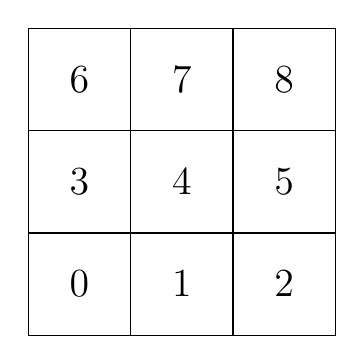
\begin{tikzpicture}[scale=1.3]
			\foreach \x in {0,...,2}{
				\foreach \y in {0,...,2}{
					\draw [draw=black] (\x, \y) rectangle (\x +1 ,\y + 1);
				}
			}
			\node at (0.5,0.5) {\Large 0};
			\node at (1.5,0.5) {\Large 1};
			\node at (2.5,0.5) {\Large 2};
			
			\node at (0.5,1.5) {\Large 3};
			\node at (1.5,1.5) {\Large 4};
			\node at (2.5,1.5) {\Large 5};
			
			\node at (0.5,2.5) {\Large 6};
			\node at (1.5,2.5) {\Large 7};
			\node at (2.5,2.5) {\Large 8};
			\end{tikzpicture}
		\end{column}
	
		\begin{column}{0.5\textwidth}
			\centering
			\vspace{-4cm}
			\begin{lstlisting}
tasks = {(0,1), (1,2,) ...,
	(0,3), (3,6), ...,
	(0,4), (1,5), ...,
	(3,1), (4,2), ...}
			\end{lstlisting}
		\end{column}
	\end{columns}

	
\end{frame}

\begin{frame}[fragile]
	\frametitle{Approach 2- Thread oriented 2D task model}
	\large
	\begin{itemize}
		\item Split up giant "`task pool"' into num\_threads jobs
		\item Use distribution strategy and information unavailable to scheduler (computing cost of each cell interaction) to distribute workload evenly
		\item Give one job to each thread
		\item Requires reduction
		\item Just one fork and join needed
	\end{itemize}



\begin{columns}
	\begin{column}{0.5\textwidth}
		\centering
			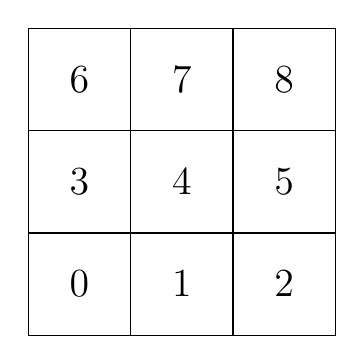
\begin{tikzpicture}[scale=1.3]
	\foreach \x in {0,...,2}{
		\foreach \y in {0,...,2}{
			\draw [draw=black] (\x, \y) rectangle (\x +1 ,\y + 1);
		}
	}
	\node at (0.5,0.5) {\Large 0};
	\node at (1.5,0.5) {\Large 1};
	\node at (2.5,0.5) {\Large 2};
	
	\node at (0.5,1.5) {\Large 3};
	\node at (1.5,1.5) {\Large 4};
	\node at (2.5,1.5) {\Large 5};
	
	\node at (0.5,2.5) {\Large 6};
	\node at (1.5,2.5) {\Large 7};
	\node at (2.5,2.5) {\Large 8};
	\end{tikzpicture}
	\end{column}
	
	\begin{column}{0.5\textwidth}
		\centering
		\vspace{-4cm}
		\begin{lstlisting}
tasks = {{(0,1), (0,3), (3,6) ...},
	{(1,2), (0,4), ...}
	...
}
		\end{lstlisting}
	\end{column}
\end{columns}
	
\end{frame}

\begin{frame}
	\frametitle{Approach 3- Color oriented 2D task model}
	\large
	\begin{itemize}
		\item You need 13 "`lines"' in the Cell-Algorithm to cover all neighbouring cell-interactions
		\item Idea: split up every line into 2 sets of edges to get 26 sets of edges that can be fully parallelized
		\item Fork and join 26 times
		\item No reduction required; no race condition in any of the 26 iterations possible
	\end{itemize}

\begin{columns}
	\begin{column}{0.5\textwidth}
		\centering
		
		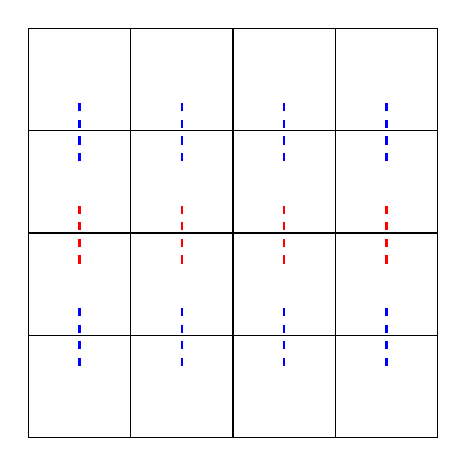
\begin{tikzpicture}[scale=1.3]
			\foreach \i in {0,...,4}{
				\draw (0,\i) --  (4,\i);
				\draw (\i, 0) -- (\i,4);
			}
			
			\foreach \y in {0,2}{
				\foreach \x in {0,...,3}{
					\draw[blue, dashed, thick](\x + 0.5, \y + 0.7) --(\x + 0.5, \y + 1.3);	
				}
			}
			
			\foreach \y in {1}{
				\foreach \x in {0,...,3}{
					\draw[thick, red, dashed, thick](\x + 0.5, \y + 0.7) --(\x + 0.5, \y + 1.3);	
				}
			}
		\end{tikzpicture}
	\end{column}
	
	\begin{column}{0.5\textwidth}
		
		\centering
		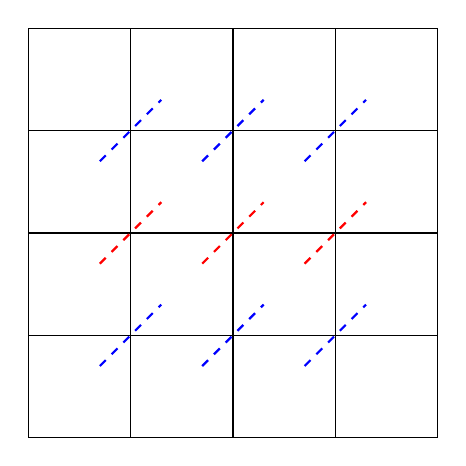
\begin{tikzpicture}[scale=1.3]
			\foreach \i in {0,...,4}{
				\draw (0,\i) --  (4,\i);
				\draw (\i, 0) -- (\i,4);
			}
			
			\foreach \y in {0,2}{
				\foreach \x in {0,...,2}{
					\draw[blue, dashed, thick](\x + 0.7, \y + 0.7) --(\x + 1.3, \y + 1.3);	
				}
			}
			
			\foreach \y in {1}{
				\foreach \x in {0,...,2}{
					\draw[red, dashed, thick](\x + 0.7, \y + 0.7) --(\x + 1.3, \y + 1.3);	
				}
			}
		
			%\foreach \y in {1 ,2, 3, 4}{
			%	\foreach \x in {0,...,3}{
				%		\draw[dashed, thick](\x + 0.7, \y + 0.3) --(\x + 1.3, \y - 0.3);	
				%	}
			%}
		\end{tikzpicture}
	\end{column}
\end{columns}
\end{frame}

\begin{frame}[fragile]
	\frametitle{Approach 3- Color oriented 2D task model}
	
	\begin{columns}
		\begin{column}{0.5\textwidth}
			\centering
			
			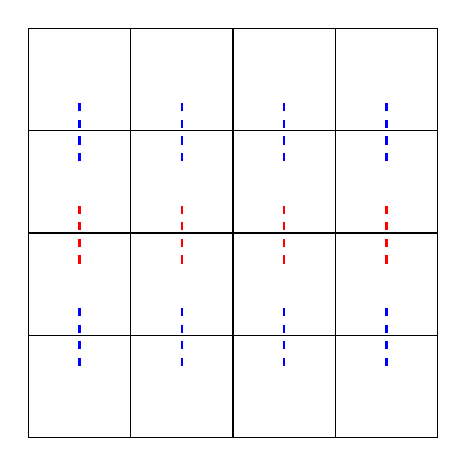
\begin{tikzpicture}[scale=1.3]
				\foreach \i in {0,...,4}{
					\draw (0,\i) --  (4,\i);
					\draw (\i, 0) -- (\i,4);
				}
				
				\foreach \y in {0,2}{
					\foreach \x in {0,...,3}{
						\draw[blue, dashed, thick](\x + 0.5, \y + 0.7) --(\x + 0.5, \y + 1.3);	
					}
				}
				
				\foreach \y in {1}{
					\foreach \x in {0,...,3}{
						\draw[thick, red, dashed, thick](\x + 0.5, \y + 0.7) --(\x + 0.5, \y + 1.3);	
					}
				}
			\end{tikzpicture}
		\end{column}
		
		\begin{column}{0.5\textwidth}
			
			\centering
			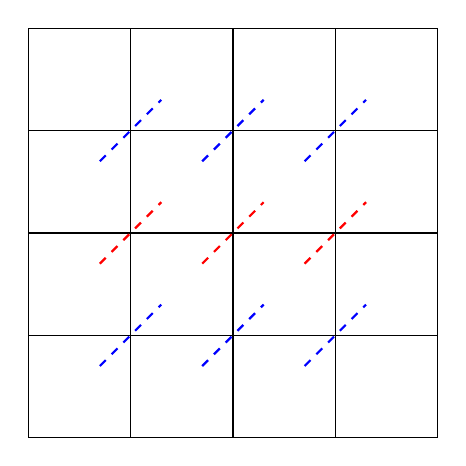
\begin{tikzpicture}[scale=1.3]
				\foreach \i in {0,...,4}{
					\draw (0,\i) --  (4,\i);
					\draw (\i, 0) -- (\i,4);
				}
				
				\foreach \y in {0,2}{
					\foreach \x in {0,...,2}{
						\draw[blue, dashed, thick](\x + 0.7, \y + 0.7) --(\x + 1.3, \y + 1.3);	
					}
				}
				
				\foreach \y in {1}{
					\foreach \x in {0,...,2}{
						\draw[red, dashed, thick](\x + 0.7, \y + 0.7) --(\x + 1.3, \y + 1.3);	
					}
				}
				
				%\foreach \y in {1 ,2, 3, 4}{
					%	\foreach \x in {0,...,3}{
						%		\draw[dashed, thick](\x + 0.7, \y + 0.3) --(\x + 1.3, \y - 0.3);	
						%	}
					%}
			\end{tikzpicture}
		\end{column}
	\end{columns}

	\begin{lstlisting}
				tasks = {{vertical blue tasks},
					{vertial red tasks},
					{diagonal blue tasks},
					{diagonal red tasks},
					{other diagonal blue tasks},
					...
				};
	\end{lstlisting}
\end{frame}
	

\begin{frame}
	\frametitle{Approach 4- 3D task model}
	\large
	\begin{itemize}
		\item Combination of thread oriented and color oriented 2D approaches
		\item Split up tasks into 26 fully parallelizable blocks
		\item Split those blocks into num\_threads jobs; use a distribution strategy to balance workload
		\item No reduction required
		\item 26 forks and joins needed
	\end{itemize}

\end{frame}

\begin{frame}
	
	\frametitle{Approach Comparison}
	\large
	\setlength\tabcolsep{0.5cm}
	\def\arraystretch{1.5}
	\begin{tabularx}{\linewidth}{>{\hsize=.25\hsize}X|>{\hsize=.25\hsize}X|>{\hsize=.25\hsize}X|>{\hsize=.25\hsize}X}	
		
		1D Tasks & 2D thread tasks
						\begin{tabular}{l|l}
							\hspace{-0.8cm}Greedy & Round Robin\\
						\end{tabular}& 2D colored tasks & 3D tasks  
					\begin{tabular}{l|l}
						\hspace{-0.8cm}Greedy & Round Robin\\
					\end{tabular}\\
		\hline
		\textcolor{black}{Simplest approach} & 
		\textcolor{black}{$+$ Potentially better scheduling than 1D tasks} &
		\textcolor{black}{$+$ Limit for parallelization corresponds to theoretical limit given by the problem} &
		\textcolor{black}{$+$ Potential to get the best out of both "`2D worlds"'}
		\\ 

		
		
		
		\textcolor{black}{$+$ Just one fork and join needed} & 
		\textcolor{black}{$+$ Just one fork and join needed} &
		\textcolor{black}{$-$ 26 forks and joins needed} &
		\textcolor{black}{$-$ 26 forks and joins needed} \\
		
		\textcolor{black}{$-$ Reduction needed} & 
		\textcolor{black}{$-$ Reduction needed} &
		\textcolor{black}{$+$ No reduction needed}&
		\textcolor{black}{$+$ No reduction needed} \\	
	\end{tabularx}
\end{frame}

\begin{frame}
	\frametitle{Speedup of the 3D task model (local build)}
		\begin{figure}
			\centering
			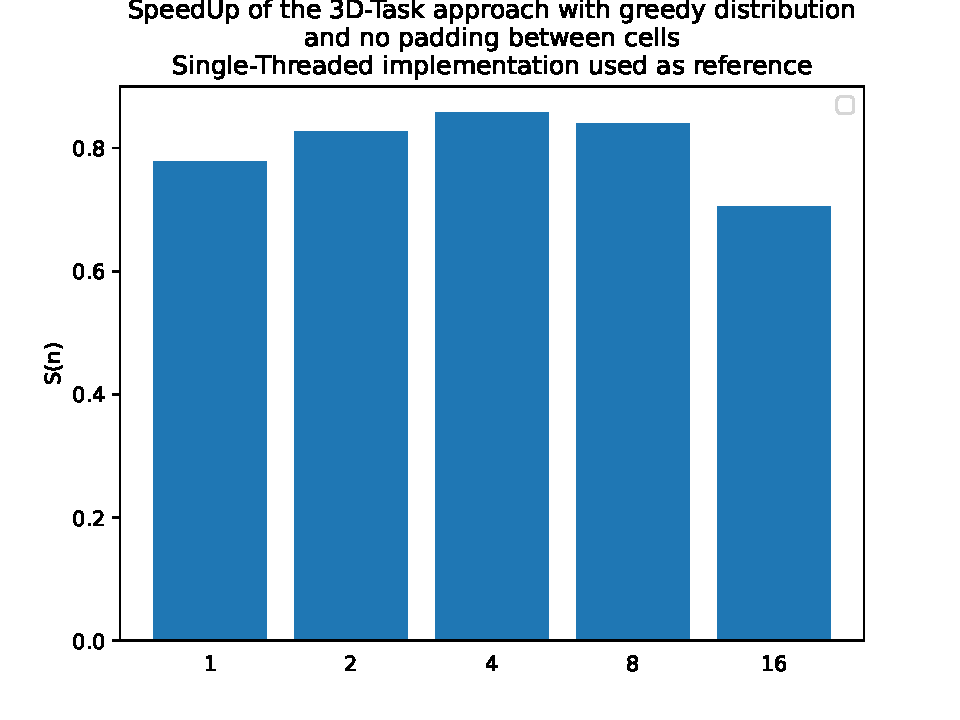
\includegraphics[width=0.6\textwidth]{speedup_3D_st_comp}
			\label{fig:speedup3dstcomp}
		\end{figure}
\end{frame}


\begin{frame}
	\frametitle{What happened?}
	\begin{figure}
		\centering
		%\includegraphics[width=\linewidth]{flame_graph_3d_problem}
		\includegraphics[width=\linewidth]{3D_multithreading_issue_table}
		%\label{fig:flamegraph3dproblem}
		\label{fig:3dmultithreadingissuetable}
	\end{figure}
	\large
\begin{itemize}
	\setlength\itemsep{1em}
	\item As you can see we only use a fraction of our time actually computing forces
	\item The majority of time is spent with OMP overhead
	\item Our conclusion: dividing the workload by $num\_threads\cdot26$ doesn't leave enough tasks in each job	
\end{itemize}
\end{frame}

\begin{frame}
	\frametitle{Speedup of the 1D approach (local build)}
	\begin{figure}
		\centering
		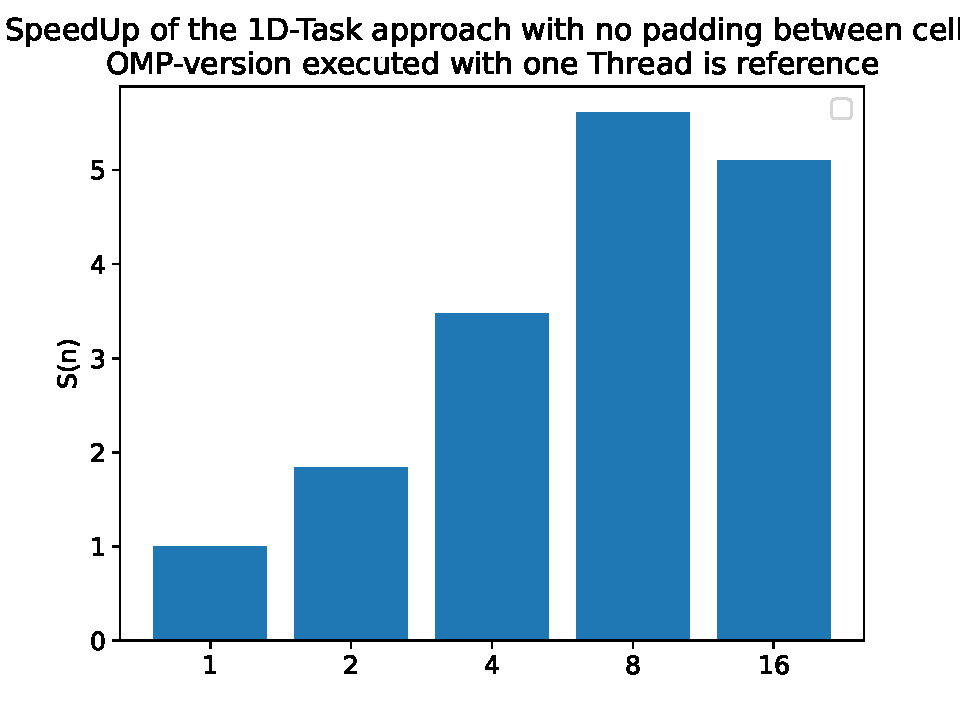
\includegraphics[width=0.57\linewidth]{speedup_1D_omp_comp}
		\label{fig:speedup1dompcomp}
	\end{figure}
	
\end{frame}

\begin{frame}
	\frametitle{Speedups of the 2D approaches (build on cluster)}
	\begin{columns}
		
	\begin{column}{0.5\linewidth}
		\begin{figure}
			\centering
			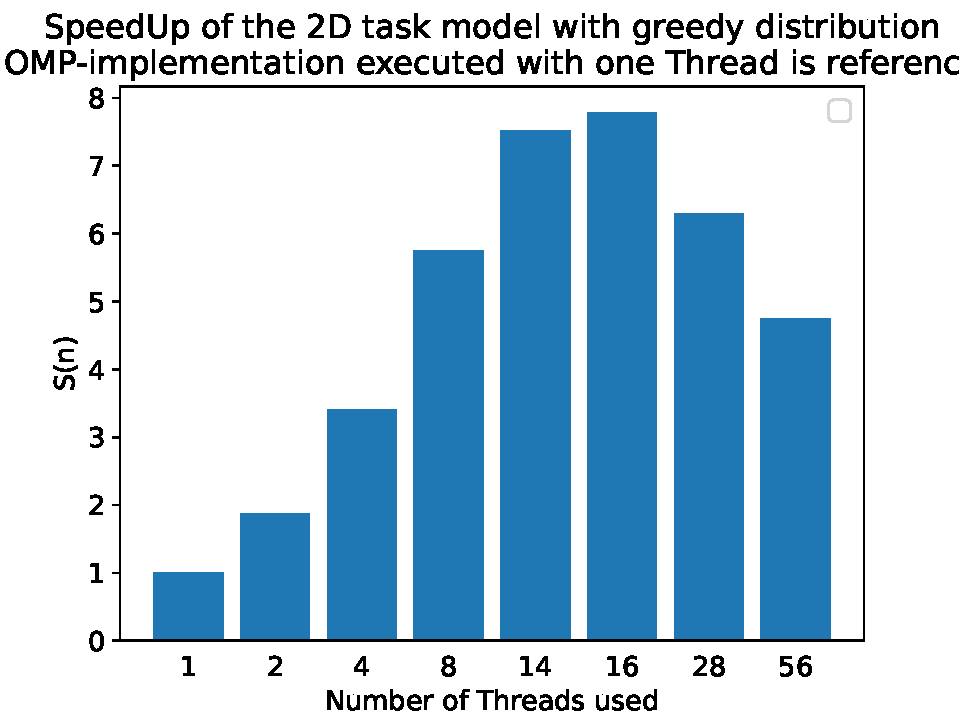
\includegraphics[width=\linewidth]{cluster2DGreedyBarGraph}
			\label{fig:cluster2dgreedybargraph}
		\end{figure}
		
	\end{column}
	
	\begin{column}{0.5\linewidth}
		\begin{figure}
			\centering
			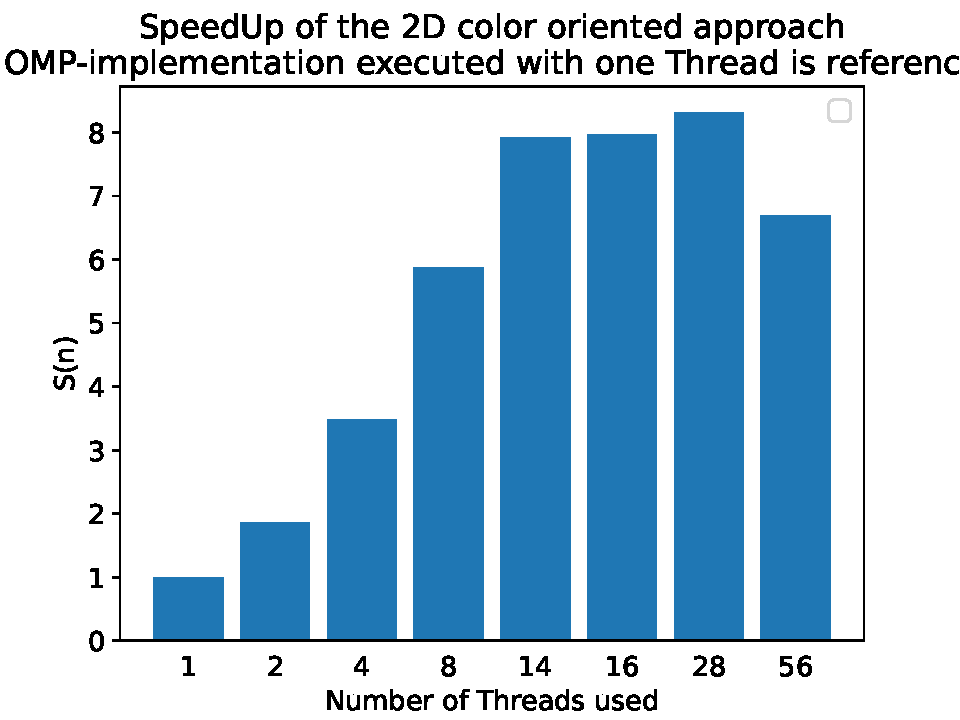
\includegraphics[width=\linewidth]{cluster2DColorBarGraph}
			\label{fig:cluster2dcolorbargraph}
		\end{figure}
	\end{column}
	\end{columns}	
\end{frame}

\begin{frame}
	\frametitle{All approaches in comparison (local build)}
	
	\begin{figure}
		\centering
		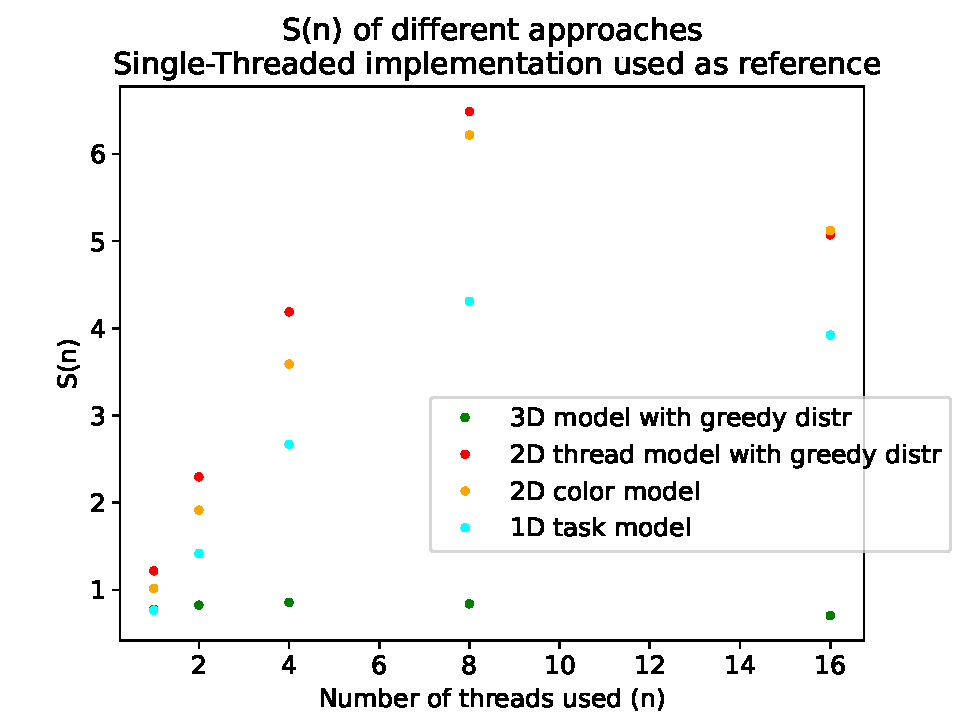
\includegraphics[width=0.55\linewidth]{speedups_all_approaches}
		%\caption{}
		\label{fig:speedupsallapproaches}
	\end{figure}
	
	
\end{frame}

\begin{frame}
	\frametitle{The price of padding}
	\vspace{0.8cm}
	\begin{columns}
		\begin{column}{0.4\linewidth}
			\large
			\begin{itemize}
				\setlength\itemsep{1em}
				\item As you can see padding adds a measurable overhead
				\item Even in cases where we expected false sharing to occur disabling padding gave a performance boost
				\item $\implies$ no padding became the default option
			\end{itemize}
			
		\end{column}
		\begin{column}{0.6\linewidth}
			\vspace{-1.6cm}
				\begin{figure}
				\centering
				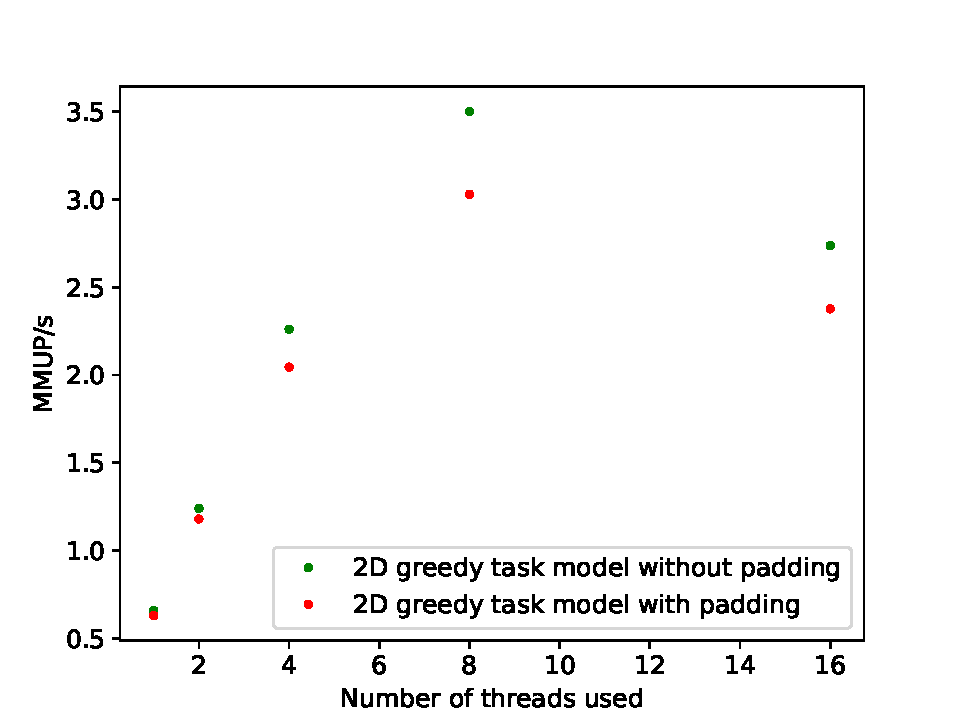
\includegraphics[width=\linewidth]{2DPaddingComp}
				%\caption{}
				\label{fig:2dpaddingcomp}
			\end{figure}
		\end{column}
	\end{columns}
\end{frame}

\begin{frame}
	\frametitle{Comparing distribution strategies}
	\begin{columns}
		\begin{column}{0.4\linewidth}
			\large
			\begin{itemize}
				\setlength\itemsep{1em}
				\item We did not manage to create a realistic scenario where Round Robin was better than the Greedy distribution
				\item $\implies$ Greedy distribution became the default option
			\end{itemize}
			
		\end{column}
		\begin{column}{0.6\linewidth}
			
		\end{column}
	\end{columns}
\end{frame}

\begin{frame}
	\frametitle{Analyzing the speedup pleateau}
	\large
	Observations:
	\vspace{-0.3cm}
	\begin{itemize}
		\item<1-> Behaviour occurs with and without padding
		\item<2-> Number of threads needed to reach speedup maximum varies from computer to computer
		\item<3-> Changing the workload per iteration step also changes the speedup maximum
		\item<4-> The more threads you add the more runtime gets used for OMP overhead methods
	\end{itemize}
	\pause
	\pause
	\pause
	\pause

	Conclusion: \\
	Not checking whether an additional thread has enough workload to be created $\implies$ creating threads where the speedup gets consumed by the OMP overhead
	
\end{frame}

\begin{frame}
	%TODO: velocity and position omp not in use since it was slower
	\frametitle{Additional parallelizations}
	\large
	Parallelization of:
	\begin{itemize}
		\item \textbf{Bounds handling}: Slight performance increase
		\item \textbf{Velocity calculation}: Performance decrease (only num\_particles operations per iteration)
		\item \textbf{Position calculation}: Performance decrease (only num\_particles operations per iteration)
	\end{itemize}
	with no design decisions worth mentioning.
	
	\vspace{0.5cm}
	
	$\implies$ no additional parallelization of other code areas with comparably small workloads
\end{frame}

\begin{frame}
	\frametitle{NanoFlow}
	
\end{frame}


\begin{frame}
	\frametitle{Issues, bugs and other timesinks}
	\large
	\begin{itemize}
		\setlength\itemsep{1em}
		\item[-]<1-> 	Our Computation of position
		\begin{equation}
			x_i(t_{n+1}) = x_i(t_n) + \Delta t \cdot v_i(t_n) + (\Delta t)^2 \cdot \frac{F_i(t_{\textcolor{red}{n-1}})}{2m_i}
		\end{equation}
		turned out to be the bug with the worst characters changed / time spent ratio.
		\item[-]<2-> Understanding the vtune-output of the 3D approach took a considerable amount of time. Looking back at it we don't really know why.
		%\item[-]<3-> Compiling with -O3 flag lead to faulty behaviour in combination with enums.
	\end{itemize}
	\pause
\end{frame}

\begin{frame}
	\PraesentationBildUhrenturm
	%\PraesentationStartseiteFlaggen
\end{frame}

%\begin{frame}
%	\frametitle{The faulty -O3 compilation}
%	\begin{figure}
%		\centering
%		\includegraphics[width=0.6\linewidth]{faulty_O3}
%		\label{fig:faultyo3}
%	\end{figure}
%	\large
%	\vspace{-0.7cm}
%	\centering
%	As you can see the thermoMode is set to pipeMode but he still enters the if-clause	
%\end{frame}


\begin{frame}
	\frametitle{Choosing a parallelization implementation}
	\large
	\begin{enumerate}
		%\setlength\itemsep{1em}
		
		\item \texttt{mkdir build}, \texttt{cd build} 
		\item Pick one: \texttt{cmake ..}, \texttt{cmake -Dround\_robin\_distr=1 ..}, \texttt{cmake -Dtask\_oriented\_2d=1 ..},\\ 
		\texttt{cmake -Done\_dim\_tasks=1 ..},   \texttt{cmake -Dthree\_dim\_tasks=1 ..},\\ 
		\texttt{cmake -Dthree\_dim\_tasks=1 -Dround\_robin\_distr=1 ..}
		
		\item \texttt{make}
		\item  \texttt{./MolSim [path to input file]} for normal execution or \\ \texttt{./MolSim [path to input file] -bench file -i [number of iterations]} to use benchmark mode 
	\end{enumerate}
\end{frame}

\begin{frame}
	\frametitle{The result}
	%TODO: insert video
	\begin{figure}[h!]
		\centering    
		\movie[label=show3,width=0.7\textwidth,poster
		,autostart,showcontrols,loop] 
		{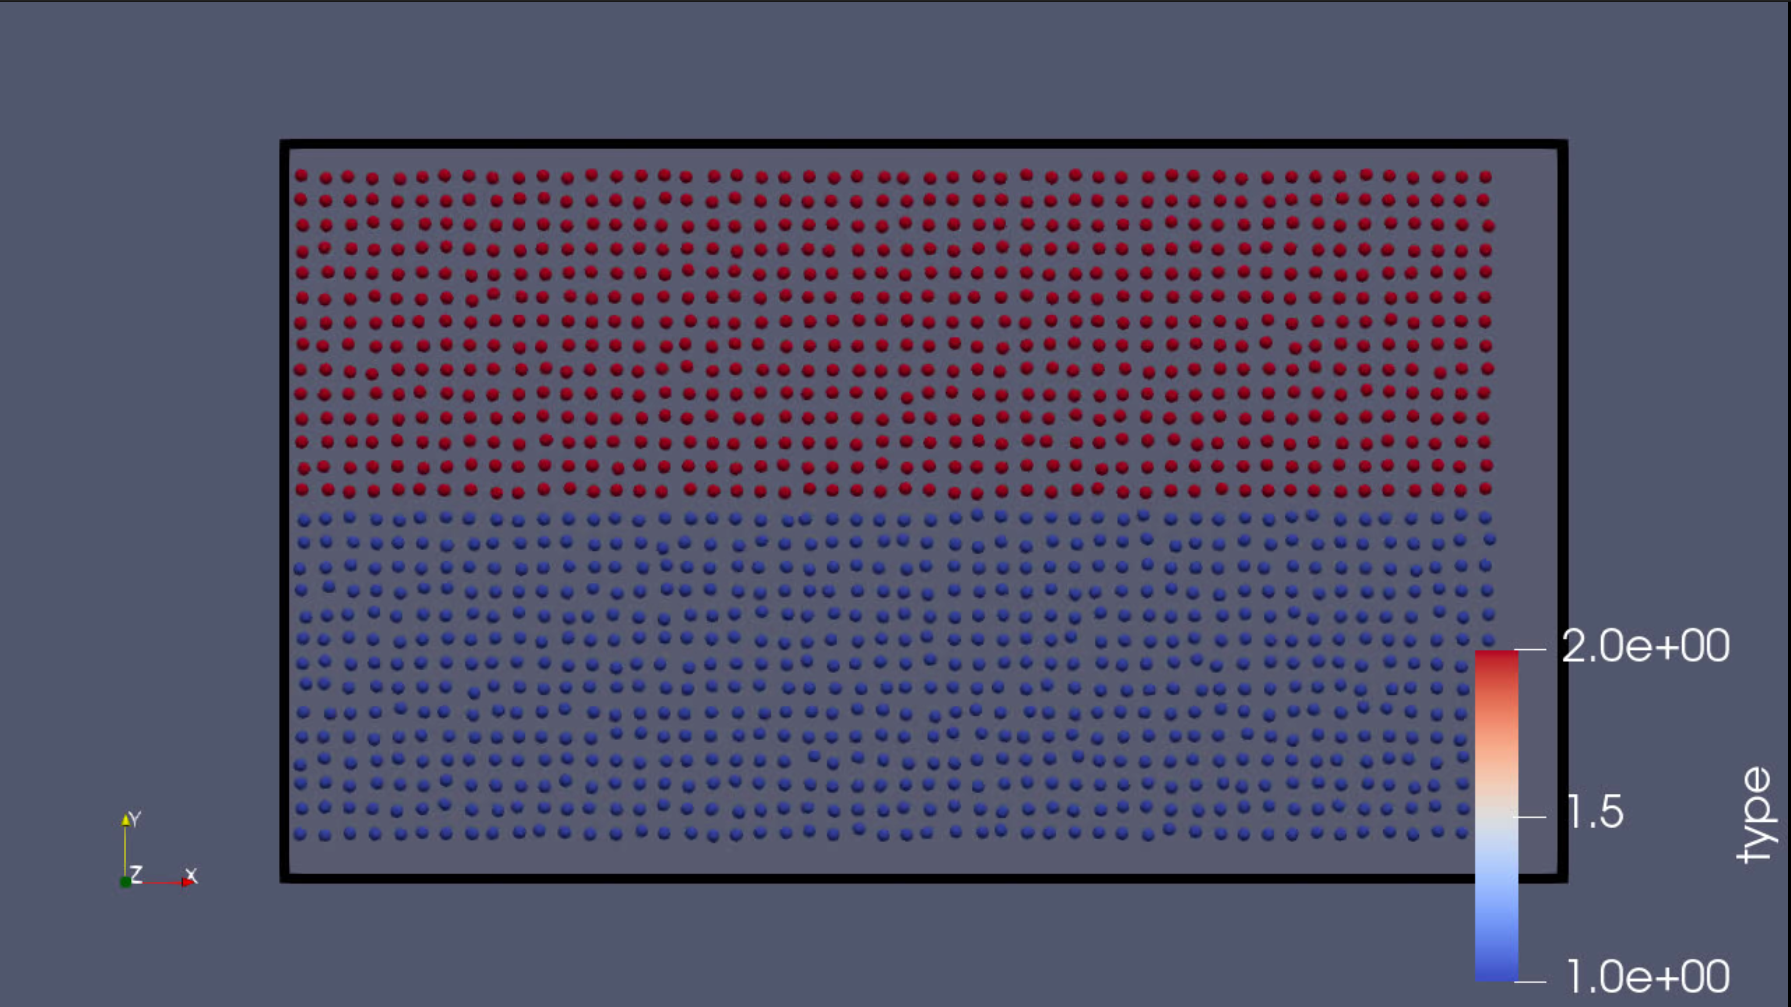
\includegraphics[width=0.7\textwidth]{small_rti.png}}{small_rti_broken.ogx}
		%\caption{caption}
	\end{figure} 
\end{frame}


\begin{frame}
	\frametitle{Additional Graphs}
	\PraesentationBildUhrenturm
	%\PraesentationStartseiteFlaggen
\end{frame}

\begin{frame}
	\frametitle{Local builds}
	\vspace{0.8cm}
	\begin{columns}
		\begin{column}{0.4\linewidth}
			\large
			Since the cluster was very crowded we let some measurements run on a local computer.
			
			Hardware details:
			
			\texttt{i7 12700 KF @ 4,7 GHz, 64 GB RAM @ 3200 MT/s}
		\end{column}
		\begin{column}{0.6\linewidth}
			content...
		\end{column}
	\end{columns}
	
	
	
	%\PraesentationStartseiteFlaggen
\end{frame}


\begin{frame}
	\frametitle{Small Rayleigh-Taylor instability}
	
	\begin{figure}[h!]
		\centering    
		\movie[label=show3,width=0.70\textwidth,poster
		,autostart,showcontrols,loop] 
		{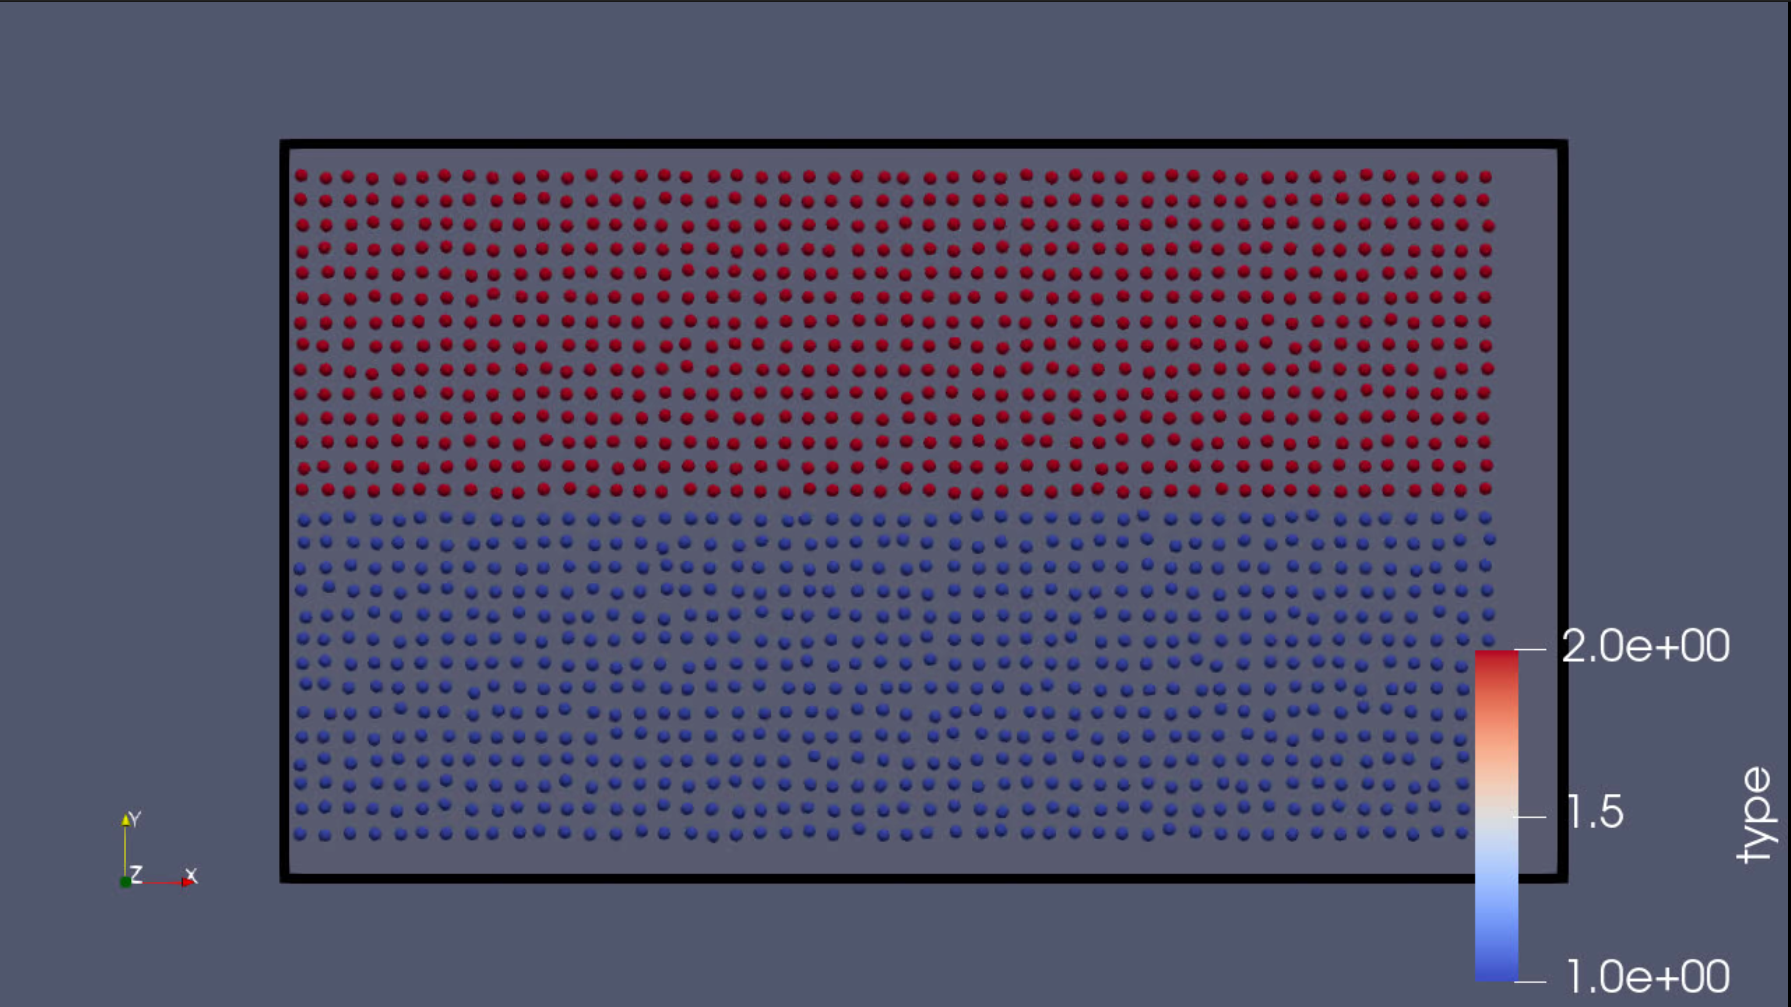
\includegraphics[width=0.70\textwidth]{small_rti.png}}{small_rti.mp4}
		%\caption{caption}
	\end{figure} 
	
\end{frame}

\begin{frame}
	\frametitle{Rayleigh-Taylor instability}
	\begin{figure}[h!]
		\centering    
		\movie[label=show3,width=0.75\textwidth,poster
		,autostart,showcontrols,loop] 
		{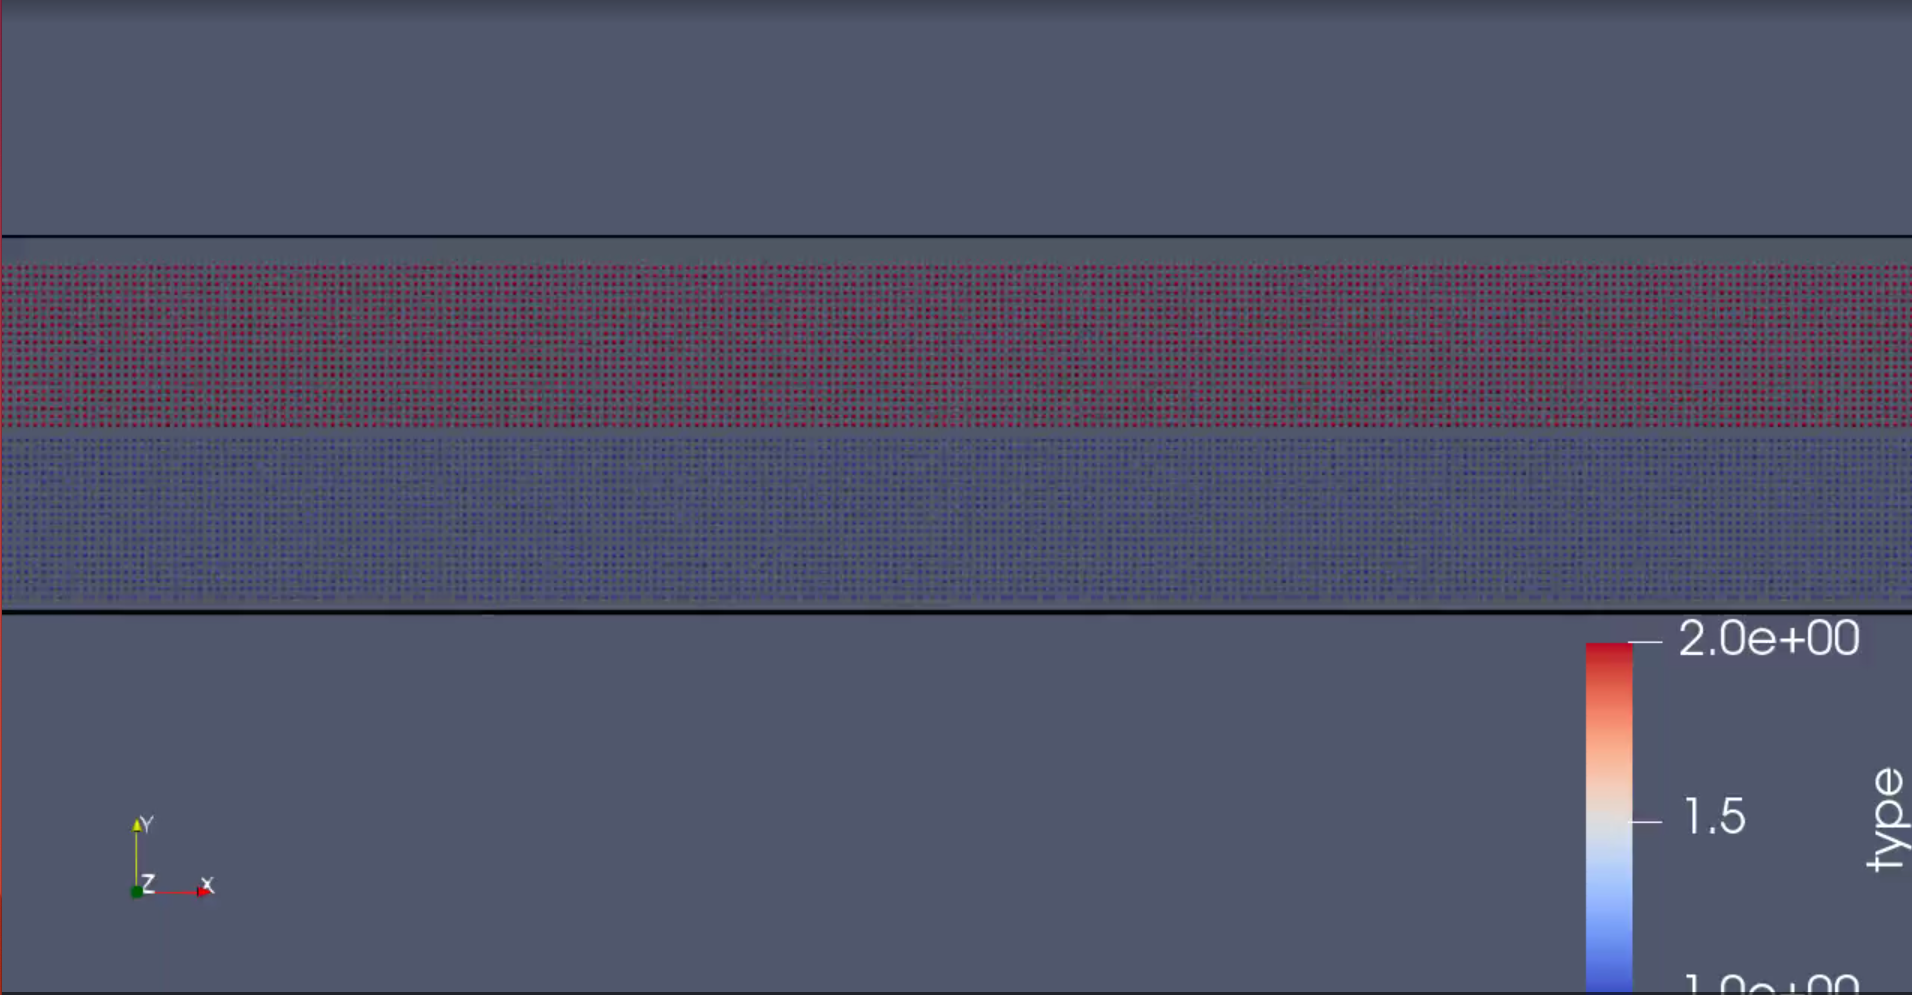
\includegraphics[width=0.75\textwidth]{large_rti.png}}{large_rti.mp4}
		%\caption{caption}
	\end{figure} 
\end{frame}

\begin{frame}
	\frametitle{Falling drop}
	\begin{figure}[h!]
		\centering    
		\movie[label=show3,width=0.70\textwidth,poster
		,autostart,showcontrols,loop] 
		{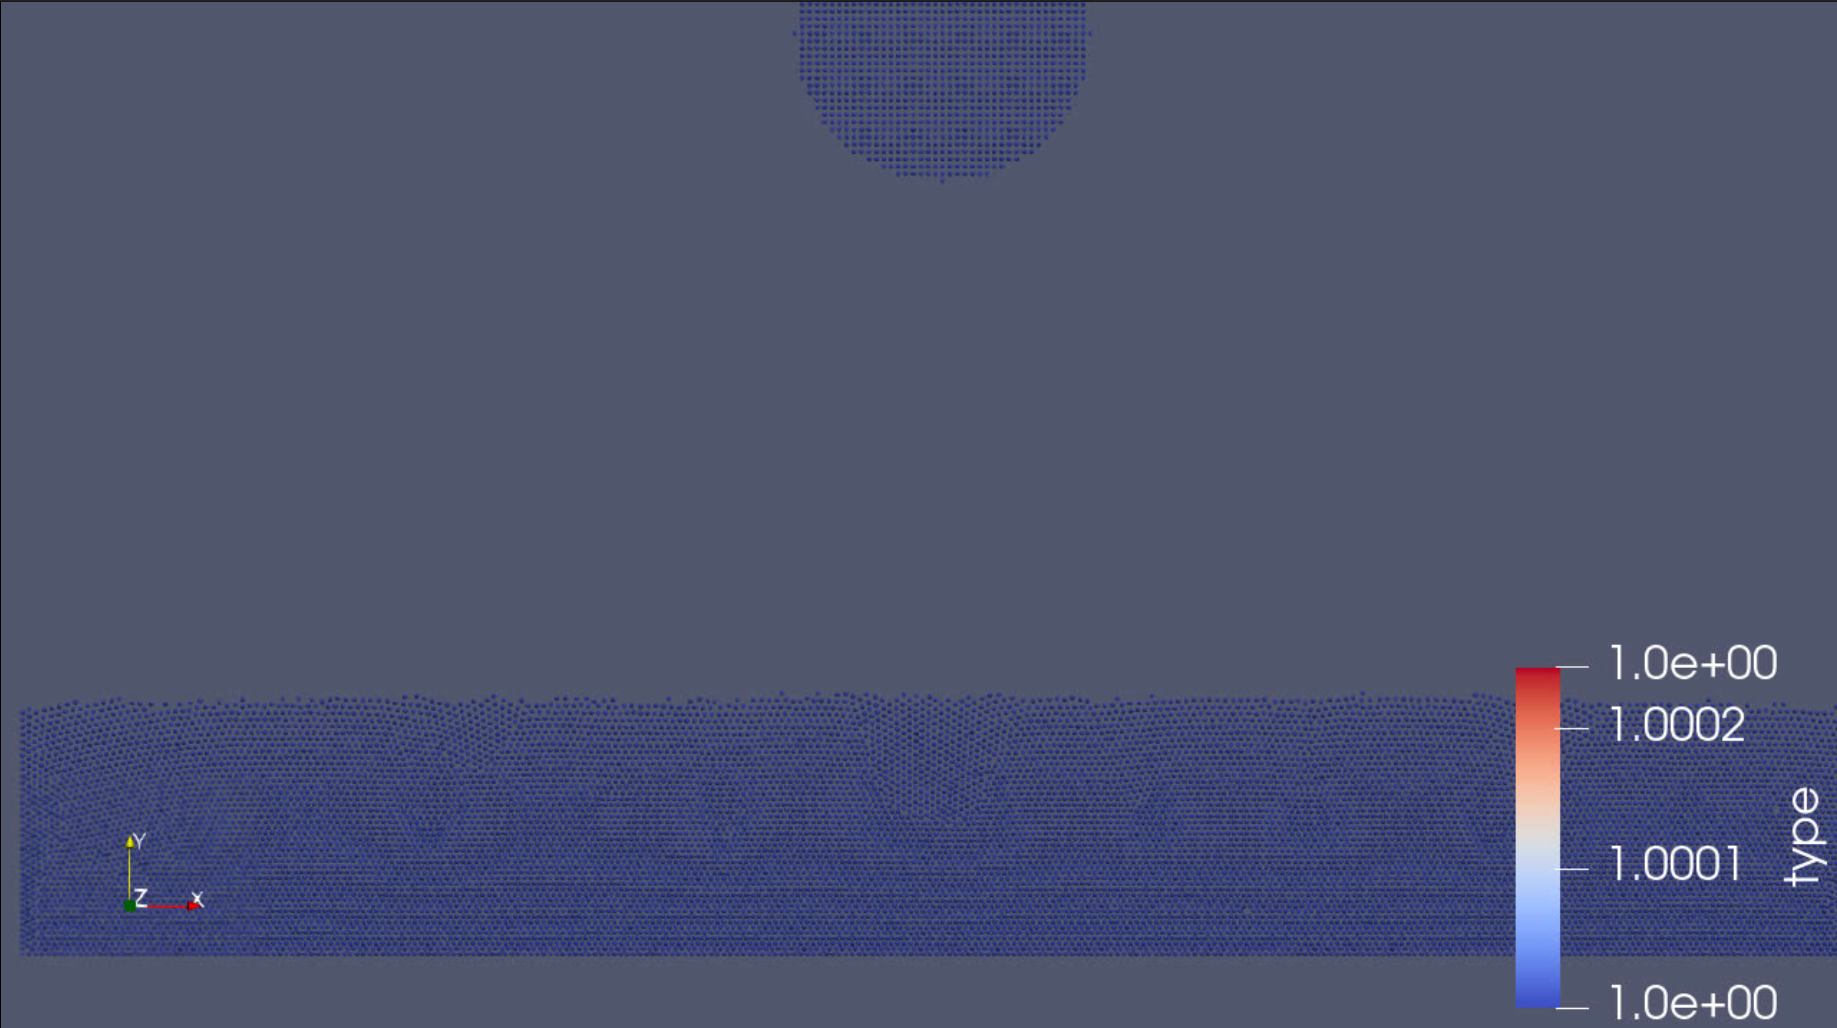
\includegraphics[width=0.70\textwidth]{falling_drop.png}}{falling_drop_out.mp4}
		%\caption{caption}
	\end{figure} 
\end{frame}



%\frame[label=blah]{
%	\begin{center}%
%		\href{run:/usr/local/bin/mplayer -fs standard-benchmark.mp4}{
%		\includegraphics[scale=0.25]
%		{Assignment2_Presentation.pdf}}

%		\includemovie{.85\textheight}{.85\textheight}{standard-benchmark.mp4}%
%	\end{center}%
%	\note{%
%		\begin{itemize}
%			\item blah
%			\item blah
%		\end{itemize}
%	}%
%}


%%%%%%%%%%%%%%%%%%%%%%%%%%%%%%%%%%%%%%%%%%%%%%%%%%%%%
%% Folie: Gültigkeit der Masterfolien              %%
%%%%%%%%%%%%%%%%%%%%%%%%%%%%%%%%%%%%%%%%%%%%%%%%%%%%%
